% !TeX encoding = UTF-8
% !TeX spellcheck = es_ES
% !TeX root = CBus.tex
%!TEX root=CBus.tex
CBus\sidenote{Usando CAN} ha sido pensado para seguir lo más fielmente posible una topologia de Bus y en los extremos una resistencia de \SI{120}{\ohm}.

\begin{figure}[H]
    \centering
    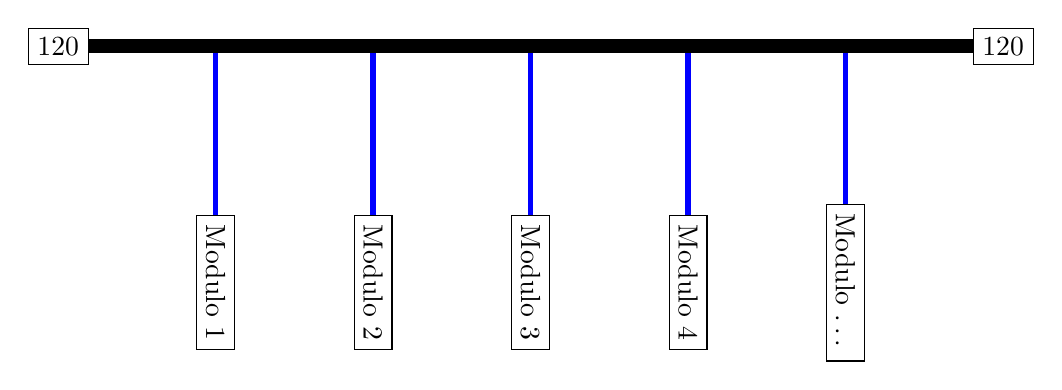
\begin{tikzpicture}
        %\draw [very thin, green]  (-6,-3) grid (6,3);
        \node at (-6,3) [rectangle,draw,align=left] (ps) {\SI{120}{\ohm}};
        \node at (6,3) [rectangle,draw,align=left] (ns) {\SI{120}{\ohm}};
        
        \node at (-4,0) [rectangle,draw,align=left,rotate=-90] (d1) {Modulo 1};
        \node at (-2,0) [rectangle,draw,align=left ,rotate=-90] (d2) {Modulo 2};
        \node at (0,0) [rectangle,draw,align=left ,rotate=-90] (d3) {Modulo 3};
        \node at (2,0) [rectangle,draw,align=left ,rotate=-90] (d4) {Modulo 4};
        \node at (4,0) [rectangle,draw,align=left ,rotate=-90] (d5) {Modulo \dots};

        \draw [line width=2, blue] (-4,3) --(d1.west);
        \draw [line width=2, blue] (-2,3) --(d2.west);
        \draw [line width=2, blue] (0,3) --(d3.west);
        \draw [line width=2, blue] (2,3) --(d4.west);
        \draw [line width=2, blue] (4,3) --(d5.west);

        \draw [line width=5] (ps.east) -- (ns.west);
    \end{tikzpicture}
    \caption{Topologia Bus}
    \label{fig:BusPuro}
\end{figure}
 
Pero a su vez permite algunas ramificaciones siempre y cuando la resitencia entre los conductores diferenciales sea aproximadamente \SI{60}{\ohm}. Ya que todos los modulos estaran conectados en paralelo a los 4 conductores.

Ademas CBUS, en general, permite utilizar otros sistemas de transporte de la informacion como puede ser
TCP, UDP, MQTT,\dots Pudiendo haber multiples Buses y segmentos unidos formando una red mayor.

\subsection{Red}
Recordemos que el objetivo de CBUS es poder controlar una maqueta de tren de forma digital. Es decir desde un
panel de mandos enviar señales para que suceda un cambio en la maqueta, o al reves, o ante un evento en la maqueta
\sidenote{Cortos, ocupacion por un tren,\dots} se actualice nuestro panel de control.

El panel de control puede ser fisico, (con lucecitas y botones) o bien puede ser una pantalla de un programa como JMRI
\sidenote{JMRI o similar, usaremos JMRI por preferencias del autor}

El caso minimo de uso CBus tendra un bus CAN con unos pocos modulos, partiendo el cable donde sea  necesario
y como mucho un CanUSB o CBusServer para conectar con JMRI. Vease \ref{fig:BusPuro}.
El caso más complejo requeria de uno o varios CBusServer cada uno conectado a uno o varios Buses CAN.
El/los CBusServer/es se comunicarian mediante TCP\sidenote{Wifi, Ethernet,\dots} entre si y distribuyendo asi los 
eventos entre todos los buses CAN.

Este ultimo caso lo podemos representar con dos buses CAN donde "Modulo 2" seria el CBusServer y
JMRI se conecta a traves de Wifi o un CanUSB.

\begin{figure}[H]
    \centering
    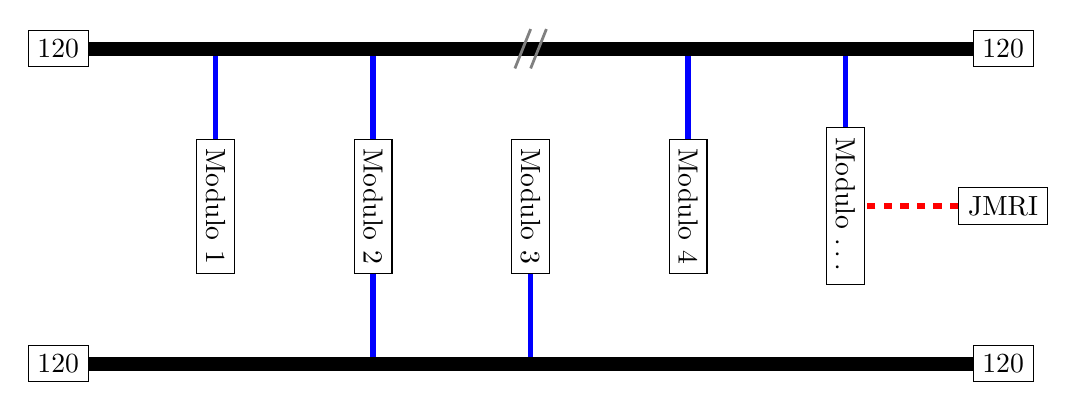
\begin{tikzpicture}
        %\draw [very thin, green]  (-6,-3) grid (6,3);
        \node at (-6,2) [rectangle,draw,align=left] (ps) {\SI{120}{\ohm}};
        \node at (6,2) [rectangle,draw,align=left] (ns) {\SI{120}{\ohm}};
        
        \node at (-6,-2) [rectangle,draw,align=left] (ps2) {\SI{120}{\ohm}};
        \node at (6,-2) [rectangle,draw,align=left] (ns2) {\SI{120}{\ohm}};

        \node at (-4,0) [rectangle,draw,align=left,rotate=-90] (d1) {Modulo 1};
        \node at (-2,0) [rectangle,draw,align=left ,rotate=-90] (d2) {Modulo 2};
        \node at (0,0) [rectangle,draw,align=left ,rotate=-90] (d3) {Modulo 3};
        \node at (2,0) [rectangle,draw,align=left ,rotate=-90] (d4) {Modulo 4};
        \node at (4,0) [rectangle,draw,align=left ,rotate=-90] (d5) {Modulo \dots};
        \node at (6,0) [rectangle,draw,align=left] (jmri) {JMRI};

        \draw [line width=2, blue] (-4,2) --(d1.west);
        \draw [line width=2, blue] (-2,2) --(d2.west);
        \draw [line width=2, blue] (-2,-2) --(d2.east);
        \draw [line width=2, blue] (0,-2) --(d3.east);
        \draw [line width=2, blue] (2,2) --(d4.west);
        \draw [line width=2, blue] (4,2) --(d5.west);

        \draw [line width=2, red, dashed] (jmri.west) --(d5.north);

        \draw [line width=5] (ps.east) -- (ns.west);
        \draw [line width=5] (ps2.east) -- (ns2.west);

        \draw [line width=1, gray] (-0.2,1.75)--(0,2.25) (0,1.75)--(0.2,2.25);


    \end{tikzpicture}
    \caption{Topologia Bus Ejemplo Red}
    \label{fig:RedEjemplo}
\end{figure}

La red CBUS es pues el conjunto de todos los dispositivos CBUS que se pueden comunicar entre si
usando el protocolo CBUS

\subsection{Segmento vs Bus vs Red vs CBusServer}
Sirva este apartado para aclarar y definir estos terminos. Puesto que esto son muy parecidos a una instalacion
TCP/IP.

\subsubsection{Bus}
Como ya se tiene una idea de lo que es la Red, empezaremos con el Bus. Siendo este el canal que permite
a todos los dispositivos conectados fisicamente al mismo comunicarse con una misma tecnologia. Hoy por Hoy solo hay dos disponibles
\sidenote{segun este punto de vista}
\begin{itemize}
    \item \textbf{CAN Bus}: Utilizar un par diferencial CAN como comunicacion.
    \item \textbf{CBusServer}: Los dispositivos se conectan mediante una conexion TCP.

\end{itemize}

De cada bus puede haber varias instancias, que no tienen que comunicarse de por si.

En resumen un Bus es un canal por lo el cual varios dispositivos se comunican entre si, sin tener que cambiar de medio.

Los buses pueden unirse o partirse, lo que hablaremos de redes o de segmentos.
Si para unirlos  es necesario una logica de transformacion de datos o de medio fisico, estaremos ante una red.

\subsubsection{Segmento}
Cuando un bus lo podamos cortar en varios trozos fisicos hablamos de segementos. En el caso de un Bus Can,
al final son dispositivos conectados entre si mediante un par de cables (H y L)\sidenote{y como mucho Vcc y GND}. Por lo que estos cables se pueden cortar en segmentos. Por otra parte CBusServer puede ejecutarse en varias maquinas (cada una una instancia) y configurase para que se hablen entre si, pero al final los clientes se conectaran a una sola maquina.

En resumen un segemento es cada una de las partes en las que un bus se puede partir sin perder la caracteristica de bus.

\subsubsection{Red}
Cuando nos encontremos con varios buses y tengamos que comunicarse entre ambos, nos encontramos con el concepto de Red. Este concepto aparece cuando al unir dos segmentos aparece alguna de estas casuisticas:
\begin{itemize}
	\item \textbf{Cambio de Medio}: Por ejemplo al pasar de CAN a TCP. Esta es una razon un poco debil, por que por ejemplo un "repetidor CAN" segun como este echo puede cambiar de medio momentanemente, o lo mismo un firewall (que no deje pasar tramas no CBUS, como OpenLCB).
Y segun lo estrictos que seamos puede ser dos buses o no.
	\item \textbf{Transformacion de datos}: Si los eventos deben ser transformados (cambiar ids, agrupar,...) 
	\item \textbf{Diferentes Funciones}: Para cada bus hemos definido una funcion diferente como puede ser eventos locales a un modulo o globales a toda la maqueta. O un bus para traccion y otro para accesorios.
\end{itemize}

En la implementacion Merg, no existe este concepto, puesto que no lo han necesitado. Tener una Red, implica tener varios buses, con la consecuencia de tener que gestionar la red. Saber para que es cada uno de los buses, asignar identificadores,\dots Pero nos abre la puerta a diseños más complejos y optimos.

\subsubsection {CBusServer}
CBusServer se corresponde con un protocolo de aplicacion sobre TCP/IP para enviar tramas CBus entre aplicaciones informaticas y como esta vision forma una tecnologia de Bus.

Pero a su vez es un Sofware de Servidor donde las diferentes aplicaciones clientes se conectan con TCP y se encarga de enviar los paquetes CBus que recibe de un cliente al resto. Este sofware puede usar el Modulo CanUSB4 de Merg y/o el Modulo CanPiHat para conectarse a una Red CBus directamente.

Este ultimo caso lo podemos representar con dos buses CAN donde "Modulo 2" seria el CBusServer y
JMRI se conecta a traves de Wifi o un CanUSB.

\subsection{Ejemplo Practico 1 - Dos Habitaciones}
Imaginemosnos una maqueta dividida en dos grandes zonas o habitaciones y con un ordenador central para  mostar el estado general de la maqueta. 

Como todo en la vida hay multiples soluciones, que implican desde un bus hasta una red de 4 o más buses.


\begin{figure}[H]
    \centering
    \begin{tikzpicture}
	\input{example/example.tikz}
   \end{tikzpicture}

    \caption{Ejemplo Practico}
    \label{fig:ejPractico}
\end{figure}
Por simplificar hemos dibujado dos ovalos, uno en cada habitacion, con dos conexiones. Simplemente representan una maqueta dividida en dos habitaciones.

Al final cada habitacion tiene sus desvios, sus detectores de ocupacion, escenografia, accesorios,\dots En la practica son dos maquetas que comparten unos puntos de conexion. 
Cada habitacion tendra su panel de control y solo estara interesada en sus propios eventos. Como mucho le interesara saber si puede enviar o recibir un tren por cada una de las conexiones.


\subsubsection{Solucion de un solo bus}
Una primera solucion podria ser tener todos los accesorios conectados a un solo bus, tanto de una zona como de la otra.

En esta solucion depende que en conjunto no se supere la longitud maxima de cableado y de dispostivos conectados \sidenote{Muchos metros y decenas de dispositivos}.
Pero aun en el muy probale caso de que no, existe otra limitacion, que es el numero de eventos y la seguridad que los eventos de una zona son ignorados por los dispositivos de la otra.\sidenote{Como mucho interesa algun error para eviar enviar trenes de una zona a la otra}


\begin{figure}[H]
    \centering
    \begin{tikzpicture}
	\input{example/example.tikz}
	\draw[red, line width=2pt](-3,-0.5)--(3,-0.5) ; 
  \end{tikzpicture}

    \caption{Ejemplo Practico - Solucion de un Bus}
    \label{fig:ejPracticoSolUnBus}
\end{figure}

\begin{mdframed}
Para Pensar: Si usamos un CBusServer para comunicar las zonas, seguimos en un bus o son tres... 
\end{mdframed}

\subsubsection{Dos buses}
Como hemos visto que hay dos zonas podemos tener cada una con su bus propio y un ordenador conectado a ambas redes. Este ordenador procesaria los eventos para mostrar en su pantalla y como mucho pasaria eventos de error en la otra zona para evitar enviar trenes de una a otra.


\begin{figure}[H]
    \centering
    \begin{tikzpicture}
	\input{example/example.tikz}
	\draw[red, line width=2pt](-3,-0.5)--(-0.5,-0.5)  (0.5,-0.5)--(3,-0.5); 
  \end{tikzpicture}

    \caption{Ejemplo Practico - Solucion de dos Buses}
    \label{fig:ejPracticoSolDosBuses}
\end{figure}

Esta solucion obliga a que el PC con el Panel Central este siempre encendido y ejecutando una logica para enviar mensajes de ocupacion/disponibildad de los tramos de interconexion.
